\documentclass[conference]{IEEEtran}
% ICME 2026/2027 regular paper: 6 pages including references, double blind.
\usepackage{cite}
\usepackage{amsmath,amssymb,amsfonts}
\usepackage{graphicx}
\usepackage{textcomp}
\usepackage{xcolor}
\usepackage{booktabs}
\usepackage{tikz}
\usetikzlibrary{arrows.meta,positioning,calc,fit,backgrounds}
\usepackage[hyphens]{url}
\graphicspath{{figures/}}

\newcommand{\dinos}{DINO-S}
\newcommand{\dinoc}{DINO-C}
\newcommand{\clips}{CLIP-S}

\begin{document}

\title{WEAVE: Escaping the Identity Shortcut in\\Lightweight Style Transfer with Wavelets}
\author{Anonymous ICME submission}
\maketitle

\begin{abstract}
Lightweight style transfer suits consumer devices, yet many compact models return an image
closer to the unchanged input than to the requested style, and standard metrics reward this
identity shortcut. We make the failure measurable with two trivial references, the
unchanged source and an unrelated target-style image, which bracket valid transfer. On three
benchmarks, eight of thirteen recent methods leave this bracket at least once. We trace the
shortcut to frequency dominance: coarse structure carries most of the training gradient but
little style information. WEAVE resolves it in the latent space of a frozen autoencoder. A Haar
transform separates structure from texture, a compact velocity network learns source-anchored
transport, and stepwise statistical alignment injects high-frequency style. With 1.04M trainable parameters and 1.4 minutes of
training on one consumer GPU, WEAVE stays inside the bracket on all benchmarks and preserves the
most content among methods that do.
\end{abstract}

\begin{IEEEkeywords}
style transfer, flow matching, wavelet decomposition, evaluation protocol, efficient generation
\end{IEEEkeywords}

\section{Introduction}
\label{sec:intro}

Artistic style transfer has moved from research demos to camera apps, creative tools, and
on-device media pipelines, where memory and latency budgets are tight. The strongest current
results come from diffusion editors and image foundation models, which reuse a billion-parameter
denoiser at every call and can require more than 60\,GB of GPU
memory~\cite{wu2025qwenimagetechnicalreport,blackforestlabs2025flux2}. Compact feed-forward and
state-space models~\cite{liu2024samst,liu2024samam,park2020cut} fit these budgets, but they raise a
question that current benchmarks rarely ask: \emph{did the output actually change style?}

\noindent\textbf{A hidden failure mode.} Content metrics such as LPIPS~\cite{zhang2018unreasonable}
and the content factor of ArtFID~\cite{wright2022artfid} are maximized by copying the input, so a
model that barely edits the source can look excellent. We therefore report two trivial outputs with
every metric (Fig.~\ref{fig:page1}): Identity (IDT) returns the source, and Target Style (TGT)
returns an unrelated image of the requested style. Valid transfer must beat IDT on style and stay
closer to the source than TGT on content. This \emph{IDT--TGT sandwich} is simple, uses raw metric
units, and is revealing: across three benchmarks, eight of thirteen recent methods fall outside it
at least once (Table~\ref{tab:main}). Some are indistinguishable from a copy in style, which we
call the \emph{identity shortcut}; others discard as much content as an unrelated painting.

\noindent\textbf{Why compact models take the shortcut.} We find the cause in the training signal
rather than in model size. When a velocity field is regressed on the full latent, the
low-frequency (LL) Haar band carries 69.5\% of the gradient energy across 5{,}000 cross-style
pairs, yet it is the \emph{least} style-discriminative band: its between-/within-style variance
ratio is 0.12, against 0.56 for the finest band HH (Fig.~\ref{fig:probes}). The objective is thus
dominated by structure that should change little, while the texture that defines style receives a
weak, easily ignored gradient. Networks that fit low frequencies first~\cite{rahaman2019spectral,xu2022frequency}
converge toward the source, and widening them does not help because both signals still share one
basis and one loss.

\noindent\textbf{Our approach.} WEAVE decides \emph{where} each signal lives before deciding how much
capacity to spend. Working on cached latents of a frozen SD1.5 VAE~\cite{rombach2022high}, a one-level
Haar transform separates structure (LL) from oriented texture (LH/HL/HH). A 1.04M-parameter
velocity network learns transport toward a source-anchored target under a down-weighted LL loss;
pooled, coordinate-free target codes steer only the LH/HL heads; and an AdaIN update aligns the
high-frequency residual after every Euler step. Training takes 82.8\,s on one RTX~3060 and stops
at an internal gradient transition, without any image evaluation.

WEAVE is the only learned model under 10M parameters that stays inside the sandwich on all three
benchmarks, and among the five methods that do, it preserves the most content, with the highest \dinoc{} on every benchmark, 11--34$\times$ fewer trainable parameters than the
other learned ones, and 11--18$\times$ faster inference than the others with a reported runtime.

\noindent\textbf{Contributions.}
(1)~\emph{Evaluation.} The IDT--TGT sandwich, a metric-agnostic protocol that exposes the identity
shortcut and content collapse, and an audit of thirteen methods under it.
(2)~\emph{Diagnosis.} A subband measurement showing that low-frequency gradient dominance, not
capacity, drives compact latent models toward identity.
(3)~\emph{Method.} Wavelet-decoupled velocity matching that assigns structure, learned texture
motion, and trajectory-level statistics to explicit subbands, with metric-free early stopping.
(4)~\emph{Evidence.} The best content preservation among valid methods at 1.04M parameters and
1.4 training minutes, supported by matched ablations, three seeds, reference-pool resampling,
zero-shot transfer, and a training-free plug-in that improves a frozen SD1.5 editor.

\begin{figure*}[t]
\centering
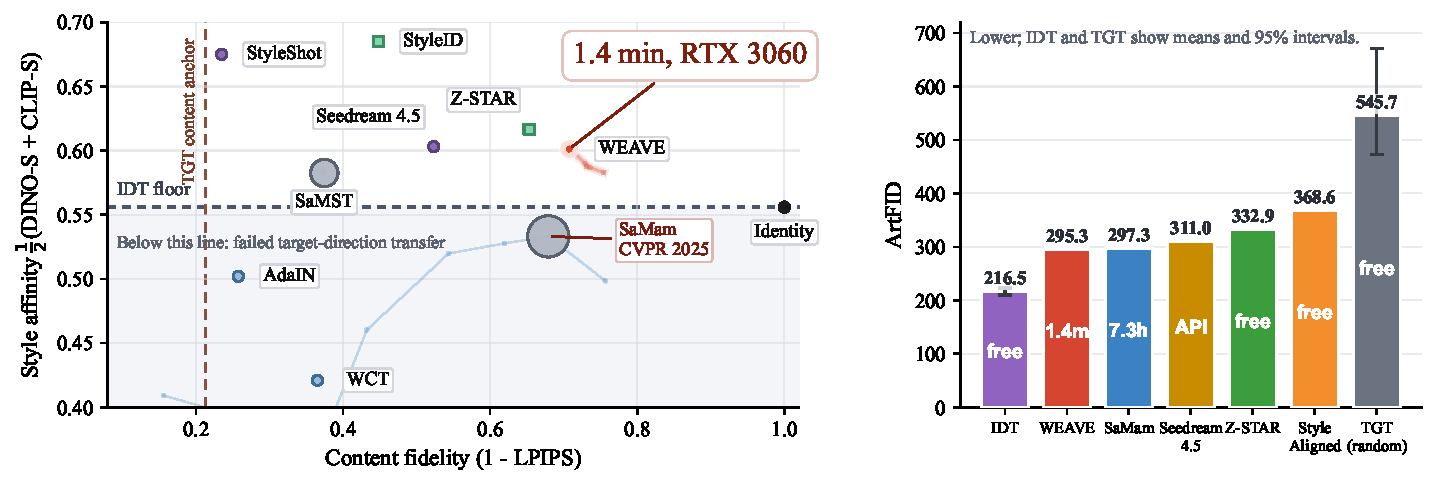
\includegraphics[width=\textwidth]{fig_distinct5_page1_summary.pdf}
\caption{IDT--TGT sandwich on D5-512. Left: style affinity versus content fidelity; bubble area
is training time. Methods below the IDT line have not moved toward the target style; methods left
of the TGT line have lost as much content as an unrelated target-style image. Right:
target-pooled ArtFID, where IDT scores best, showing why a no-op reference is needed (IDT: 95\%
bootstrap interval; TGT: 2.5--97.5 percentile over 30 reference draws).}
\label{fig:page1}
\end{figure*}

\section{Related Work}
\label{sec:related}

\noindent\textbf{Neural and statistical style transfer.} Gatys et al.\ matched Gram statistics
by optimization~\cite{gatys2015neural,gatys2016image}; AdaIN and WCT replaced it with feed-forward
moment and covariance transforms~\cite{huang2017arbitrary,li2017universal}. SANet, StyTR-2, and
AesPA-Net add attention~\cite{park2019sanet,deng2022stytr2,hong2023aespa}, CUT learns unpaired
translation by patch contrast~\cite{park2020cut}, and Mamba-based SaMST and SaMam reduce sequence
cost~\cite{liu2024samst,liu2024samam,gu2023mamba}. These methods mix structure and appearance in
one feature tensor; WEAVE restricts statistical correction to explicit frequency coordinates.

\noindent\textbf{Diffusion editors.} Latent diffusion~\cite{rombach2022high} enables SDEdit,
Prompt-to-Prompt, StyleID, StyleAligned, InST, Z-STAR, IP-Adapter, and
StyleShot~\cite{meng2021sdedit,hertz2022prompt,chung2024style,hertz2024style,zhang2023inst,lu2024zstar,ye2023ipadapter,gao2024styleshot}.
Being ``training-free'' leaves a 1B-parameter denoiser, often with inversion, in every call.
WEAVE keeps only the frozen VAE; our plug-in experiment tests the Haar operator inside such an editor.

\noindent\textbf{Flow matching and bridges.} Rectified flow and flow
matching~\cite{liu2022rectified,lipman2022flow} regress velocities along endpoint interpolations,
and Schr\"odinger-bridge solvers~\cite{debortoli2021dsb,shi2023dsbm,liu2023i2sb,su2023ddib} address
unpaired domains, but their objectives weigh all coordinates together. WEAVE changes the endpoint,
basis, and per-band weights of the same regression.

\noindent\textbf{Frequency-aware and wavelet methods.} FDIT constrains low and high frequencies
separately for translation~\cite{cai2021fdit}, FreqFlow weights frequencies for class-conditional
generation~\cite{ren2026freqflow}, and wavelets support diffusion~\cite{phung2023wavelet} and
photorealistic transfer~\cite{yoo2019photorealistic}. WEAVE uses the orthogonal Haar
basis~\cite{daubechies1992ten} \emph{inside} the transport objective, with a distinct role per band.

\begin{figure}[t]
\centering
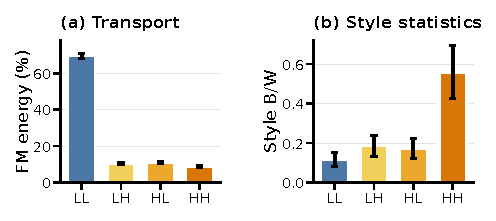
\includegraphics[width=\columnwidth]{fig_probe_combined.pdf}
\caption{Frequency probes on 5{,}000 cross-style latent pairs. (a)~Share of endpoint-displacement
energy per Haar band. (b)~Between-/within-style variance ratio of per-image band statistics.
Transport energy concentrates in LL while style separation is strongest at high frequency.}
\label{fig:probes}
\end{figure}

\section{Method}
\label{sec:method}

\begin{figure*}[t]
\centering
\resizebox{\textwidth}{!}{% WEAVE architecture (TikZ). Included by weave.tex via % WEAVE architecture (TikZ). Included by weave.tex via % WEAVE architecture (TikZ). Included by weave.tex via \input{fig_arch}.
% Needs: \usetikzlibrary{arrows.meta,positioning,calc,fit,backgrounds}
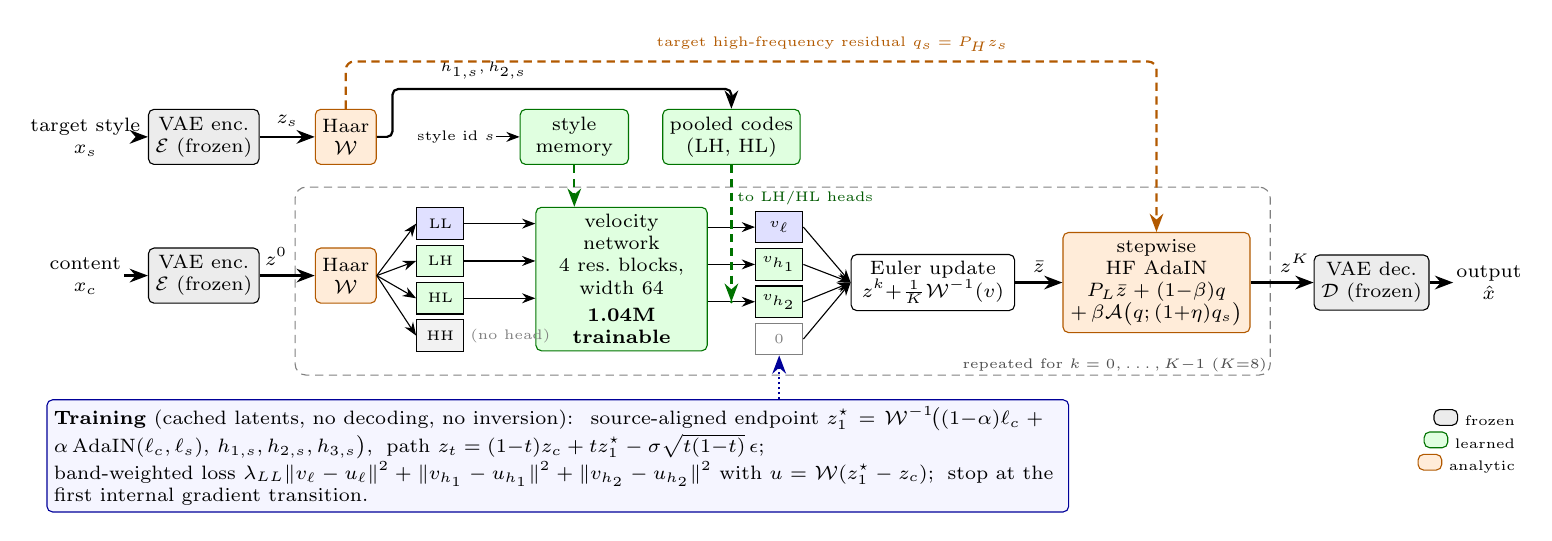
\begin{tikzpicture}[
  font=\scriptsize, >=Stealth, node distance=3mm,
  box/.style={draw, rounded corners=2pt, align=center, inner sep=2.5pt, minimum height=7mm},
  frozen/.style={box, fill=gray!15},
  learn/.style={box, fill=green!12, draw=green!45!black},
  analytic/.style={box, fill=orange!15, draw=orange!70!black},
  data/.style={align=center, inner sep=1pt},
  band/.style={draw, minimum width=6mm, minimum height=4mm, inner sep=0pt, font=\tiny},
  flow/.style={->, thick},
  cond/.style={->, densely dashed, orange!70!black, thick},
  lcond/.style={->, densely dashed, green!45!black, thick},
]
% ---------------- main inference path ----------------
\node[data] (xc) {content\\$x_c$};
\node[frozen, right=of xc] (enc) {VAE enc.\\$\mathcal E$ (frozen)};
\node[analytic, right=7mm of enc] (dwt) {Haar\\$\mathcal W$};
\node[band, fill=blue!12, right=5mm of dwt, yshift=6.6mm] (ll) {LL};
\node[band, fill=green!12, below=0.6mm of ll] (lh) {LH};
\node[band, fill=green!12, below=0.6mm of lh] (hl) {HL};
\node[band, fill=gray!10, below=0.6mm of hl] (hh) {HH};
\node[learn, right=9mm of lh, yshift=-2.3mm, minimum height=17mm, text width=20mm] (net)
  {velocity network\\4 res.\ blocks, width 64\\[2pt]\textbf{1.04M trainable}};
\node[band, fill=blue!12, right=6mm of net, yshift=6.6mm] (vll) {$v_\ell$};
\node[band, fill=green!12, below=0.6mm of vll] (vlh) {$v_{h_1}$};
\node[band, fill=green!12, below=0.6mm of vlh] (vhl) {$v_{h_2}$};
\node[band, draw=gray, text=gray, below=0.6mm of vhl] (vhh) {$0$};
\node[box, right=6mm of vlh, yshift=-2.3mm, text width=19mm] (euler)
  {Euler update\\$z^k{+}\tfrac1K\mathcal W^{-1}(v)$};
\node[analytic, right=6mm of euler, text width=22mm] (adain)
  {stepwise HF AdaIN\\$P_L\bar z+(1{-}\beta)q$\\$+\,\beta\mathcal A\big(q;(1{+}\eta)q_s\big)$};
\node[frozen, right=8mm of adain] (dec) {VAE dec.\\$\mathcal D$ (frozen)};
\node[data, right=of dec] (out) {output\\$\hat x$};

\draw[flow] (xc) -- (enc);
\draw[flow] (enc) -- node[above, pos=0.3]{$z^0$} (dwt);
\foreach \b in {ll,lh,hl,hh} \draw[->] (dwt.east) -- (\b.west);
\foreach \b in {ll,lh,hl} \draw[->] (\b.east) -- (\b.east -| net.west);
\node[font=\tiny, text=gray, anchor=west, inner sep=0.5pt] at ([xshift=0.5mm]hh.east) {(no head)};
\foreach \b in {vll,vlh,vhl} \draw[->] (\b.west -| net.east) -- (\b.west);
\foreach \b in {vll,vlh,vhl,vhh} \draw[->] (\b.east) -- (euler.west);
\draw[flow] (euler) -- node[above]{$\bar z$} (adain);
\draw[flow] (adain) -- node[above, pos=0.7]{$z^{K}$} (dec);
\draw[flow] (dec) -- (out);

\begin{scope}[on background layer]
\node[draw=black!50, densely dashed, rounded corners=4pt, inner sep=2.5mm,
      fit=(dwt)(ll)(hh)(net)(vll)(vhh)(euler)(adain)] (loop) {};
\end{scope}
\node[anchor=south east, font=\tiny, text=black!70, inner sep=1.2pt] at (loop.south east) {repeated for $k=0,\dots,K{-}1$ ($K{=}8$)};

\coordinate (mid) at ($(net.east)!0.5!(vlh.west)$);
% ---------------- style conditioning (top) ----------------
\node[data, above=12mm of xc] (xs) {target style\\$x_s$};
\node[frozen] (enc2) at (xs -| enc) {VAE enc.\\$\mathcal E$ (frozen)};
\node[analytic] (dwt2) at (xs -| dwt) {Haar\\$\mathcal W$};
\node[learn] (pool) at (xs -| mid) {pooled codes\\(LH, HL)};
\node[learn, text width=12mm] (mem) at ([xshift=-6mm]xs -| net) {style\\memory};
\draw[flow] (xs) -- (enc2);
\draw[flow] (enc2) -- node[above]{$z_s$} (dwt2);
\draw[flow, rounded corners=2pt] (dwt2.east) -- ++(2mm,0) |- ([yshift=2.5mm]mem.north) node[pos=0.75, above, font=\tiny]{$h_{1,s},h_{2,s}$} -| (pool.north);
\draw[lcond] (pool.south) -- (mid |- vhl.west);
\fill[green!45!black] (mid |- vlh.west) circle (0.6pt) (mid |- vhl.west) circle (0.6pt);
\node[font=\tiny, text=green!35!black, anchor=north west, inner sep=0.5pt] at ([xshift=0.5mm,yshift=-0.4mm]mid |- loop.north) {to LH/HL heads};
\draw[lcond] (mem.south) -- (mem.south |- net.north);
\node[font=\tiny, anchor=east, inner sep=0.5pt] (sid) at ([xshift=-3mm]mem.west) {style id $s$};
\draw[->] (sid) -- (mem);
\draw[cond, rounded corners=3pt] (dwt2.north) -- ++(0,6mm) -| node[pos=0.3, above, font=\tiny]{target high-frequency residual $q_s=P_H z_s$} (adain.north);

% ---------------- training objective (bottom) ----------------
\node[box, draw=blue!60!black, fill=blue!4, anchor=north west, text width=128mm, align=left]
  (loss) at ([yshift=-3mm]loop.south west -| xc.west)
  {\textbf{Training} (cached latents, no decoding, no inversion):\;
  source-aligned endpoint $z_1^\star=\mathcal W^{-1}\!\big((1{-}\alpha)\ell_c+\alpha\,\mathrm{AdaIN}(\ell_c,\ell_s),\,h_{1,s},h_{2,s},h_{3,s}\big)$,\;
  path $z_t=(1{-}t)z_c+t z_1^\star-\sigma\sqrt{t(1{-}t)}\,\epsilon$;\\
  band-weighted loss $\lambda_{LL}\|v_\ell-u_\ell\|^2+\|v_{h_1}-u_{h_1}\|^2+\|v_{h_2}-u_{h_2}\|^2$ with $u=\mathcal W(z_1^\star-z_c)$;\;
  stop at the first internal gradient transition.};
\draw[->, densely dotted, blue!60!black, thick] (loss.north -| vhh.south) -- (vhh.south);

\node[anchor=north east, font=\tiny, align=right] at (loss.north east -| out.east) {%
  \tikz\node[frozen, minimum height=2mm, minimum width=3mm]{};\ frozen\\[1pt]
  \tikz\node[learn, minimum height=2mm, minimum width=3mm]{};\ learned\\[1pt]
  \tikz\node[analytic, minimum height=2mm, minimum width=3mm]{};\ analytic};
\end{tikzpicture}
.
% Needs: \usetikzlibrary{arrows.meta,positioning,calc,fit,backgrounds}
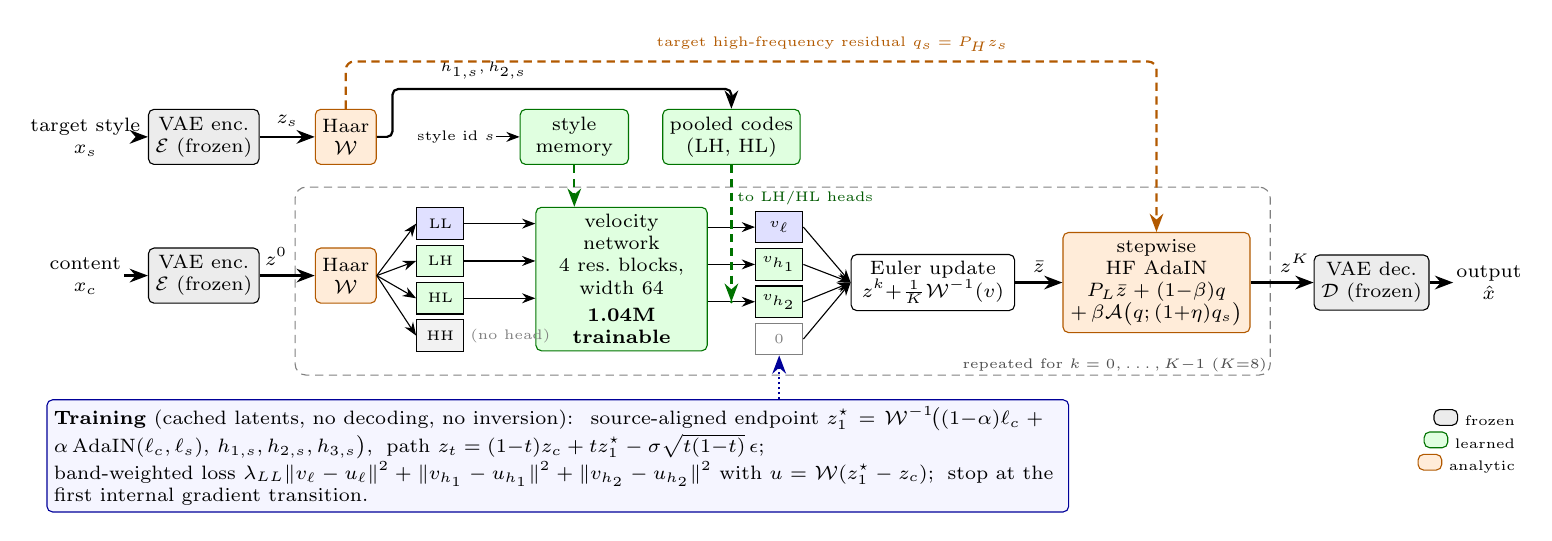
\begin{tikzpicture}[
  font=\scriptsize, >=Stealth, node distance=3mm,
  box/.style={draw, rounded corners=2pt, align=center, inner sep=2.5pt, minimum height=7mm},
  frozen/.style={box, fill=gray!15},
  learn/.style={box, fill=green!12, draw=green!45!black},
  analytic/.style={box, fill=orange!15, draw=orange!70!black},
  data/.style={align=center, inner sep=1pt},
  band/.style={draw, minimum width=6mm, minimum height=4mm, inner sep=0pt, font=\tiny},
  flow/.style={->, thick},
  cond/.style={->, densely dashed, orange!70!black, thick},
  lcond/.style={->, densely dashed, green!45!black, thick},
]
% ---------------- main inference path ----------------
\node[data] (xc) {content\\$x_c$};
\node[frozen, right=of xc] (enc) {VAE enc.\\$\mathcal E$ (frozen)};
\node[analytic, right=7mm of enc] (dwt) {Haar\\$\mathcal W$};
\node[band, fill=blue!12, right=5mm of dwt, yshift=6.6mm] (ll) {LL};
\node[band, fill=green!12, below=0.6mm of ll] (lh) {LH};
\node[band, fill=green!12, below=0.6mm of lh] (hl) {HL};
\node[band, fill=gray!10, below=0.6mm of hl] (hh) {HH};
\node[learn, right=9mm of lh, yshift=-2.3mm, minimum height=17mm, text width=20mm] (net)
  {velocity network\\4 res.\ blocks, width 64\\[2pt]\textbf{1.04M trainable}};
\node[band, fill=blue!12, right=6mm of net, yshift=6.6mm] (vll) {$v_\ell$};
\node[band, fill=green!12, below=0.6mm of vll] (vlh) {$v_{h_1}$};
\node[band, fill=green!12, below=0.6mm of vlh] (vhl) {$v_{h_2}$};
\node[band, draw=gray, text=gray, below=0.6mm of vhl] (vhh) {$0$};
\node[box, right=6mm of vlh, yshift=-2.3mm, text width=19mm] (euler)
  {Euler update\\$z^k{+}\tfrac1K\mathcal W^{-1}(v)$};
\node[analytic, right=6mm of euler, text width=22mm] (adain)
  {stepwise HF AdaIN\\$P_L\bar z+(1{-}\beta)q$\\$+\,\beta\mathcal A\big(q;(1{+}\eta)q_s\big)$};
\node[frozen, right=8mm of adain] (dec) {VAE dec.\\$\mathcal D$ (frozen)};
\node[data, right=of dec] (out) {output\\$\hat x$};

\draw[flow] (xc) -- (enc);
\draw[flow] (enc) -- node[above, pos=0.3]{$z^0$} (dwt);
\foreach \b in {ll,lh,hl,hh} \draw[->] (dwt.east) -- (\b.west);
\foreach \b in {ll,lh,hl} \draw[->] (\b.east) -- (\b.east -| net.west);
\node[font=\tiny, text=gray, anchor=west, inner sep=0.5pt] at ([xshift=0.5mm]hh.east) {(no head)};
\foreach \b in {vll,vlh,vhl} \draw[->] (\b.west -| net.east) -- (\b.west);
\foreach \b in {vll,vlh,vhl,vhh} \draw[->] (\b.east) -- (euler.west);
\draw[flow] (euler) -- node[above]{$\bar z$} (adain);
\draw[flow] (adain) -- node[above, pos=0.7]{$z^{K}$} (dec);
\draw[flow] (dec) -- (out);

\begin{scope}[on background layer]
\node[draw=black!50, densely dashed, rounded corners=4pt, inner sep=2.5mm,
      fit=(dwt)(ll)(hh)(net)(vll)(vhh)(euler)(adain)] (loop) {};
\end{scope}
\node[anchor=south east, font=\tiny, text=black!70, inner sep=1.2pt] at (loop.south east) {repeated for $k=0,\dots,K{-}1$ ($K{=}8$)};

\coordinate (mid) at ($(net.east)!0.5!(vlh.west)$);
% ---------------- style conditioning (top) ----------------
\node[data, above=12mm of xc] (xs) {target style\\$x_s$};
\node[frozen] (enc2) at (xs -| enc) {VAE enc.\\$\mathcal E$ (frozen)};
\node[analytic] (dwt2) at (xs -| dwt) {Haar\\$\mathcal W$};
\node[learn] (pool) at (xs -| mid) {pooled codes\\(LH, HL)};
\node[learn, text width=12mm] (mem) at ([xshift=-6mm]xs -| net) {style\\memory};
\draw[flow] (xs) -- (enc2);
\draw[flow] (enc2) -- node[above]{$z_s$} (dwt2);
\draw[flow, rounded corners=2pt] (dwt2.east) -- ++(2mm,0) |- ([yshift=2.5mm]mem.north) node[pos=0.75, above, font=\tiny]{$h_{1,s},h_{2,s}$} -| (pool.north);
\draw[lcond] (pool.south) -- (mid |- vhl.west);
\fill[green!45!black] (mid |- vlh.west) circle (0.6pt) (mid |- vhl.west) circle (0.6pt);
\node[font=\tiny, text=green!35!black, anchor=north west, inner sep=0.5pt] at ([xshift=0.5mm,yshift=-0.4mm]mid |- loop.north) {to LH/HL heads};
\draw[lcond] (mem.south) -- (mem.south |- net.north);
\node[font=\tiny, anchor=east, inner sep=0.5pt] (sid) at ([xshift=-3mm]mem.west) {style id $s$};
\draw[->] (sid) -- (mem);
\draw[cond, rounded corners=3pt] (dwt2.north) -- ++(0,6mm) -| node[pos=0.3, above, font=\tiny]{target high-frequency residual $q_s=P_H z_s$} (adain.north);

% ---------------- training objective (bottom) ----------------
\node[box, draw=blue!60!black, fill=blue!4, anchor=north west, text width=128mm, align=left]
  (loss) at ([yshift=-3mm]loop.south west -| xc.west)
  {\textbf{Training} (cached latents, no decoding, no inversion):\;
  source-aligned endpoint $z_1^\star=\mathcal W^{-1}\!\big((1{-}\alpha)\ell_c+\alpha\,\mathrm{AdaIN}(\ell_c,\ell_s),\,h_{1,s},h_{2,s},h_{3,s}\big)$,\;
  path $z_t=(1{-}t)z_c+t z_1^\star-\sigma\sqrt{t(1{-}t)}\,\epsilon$;\\
  band-weighted loss $\lambda_{LL}\|v_\ell-u_\ell\|^2+\|v_{h_1}-u_{h_1}\|^2+\|v_{h_2}-u_{h_2}\|^2$ with $u=\mathcal W(z_1^\star-z_c)$;\;
  stop at the first internal gradient transition.};
\draw[->, densely dotted, blue!60!black, thick] (loss.north -| vhh.south) -- (vhh.south);

\node[anchor=north east, font=\tiny, align=right] at (loss.north east -| out.east) {%
  \tikz\node[frozen, minimum height=2mm, minimum width=3mm]{};\ frozen\\[1pt]
  \tikz\node[learn, minimum height=2mm, minimum width=3mm]{};\ learned\\[1pt]
  \tikz\node[analytic, minimum height=2mm, minimum width=3mm]{};\ analytic};
\end{tikzpicture}
.
% Needs: \usetikzlibrary{arrows.meta,positioning,calc,fit,backgrounds}
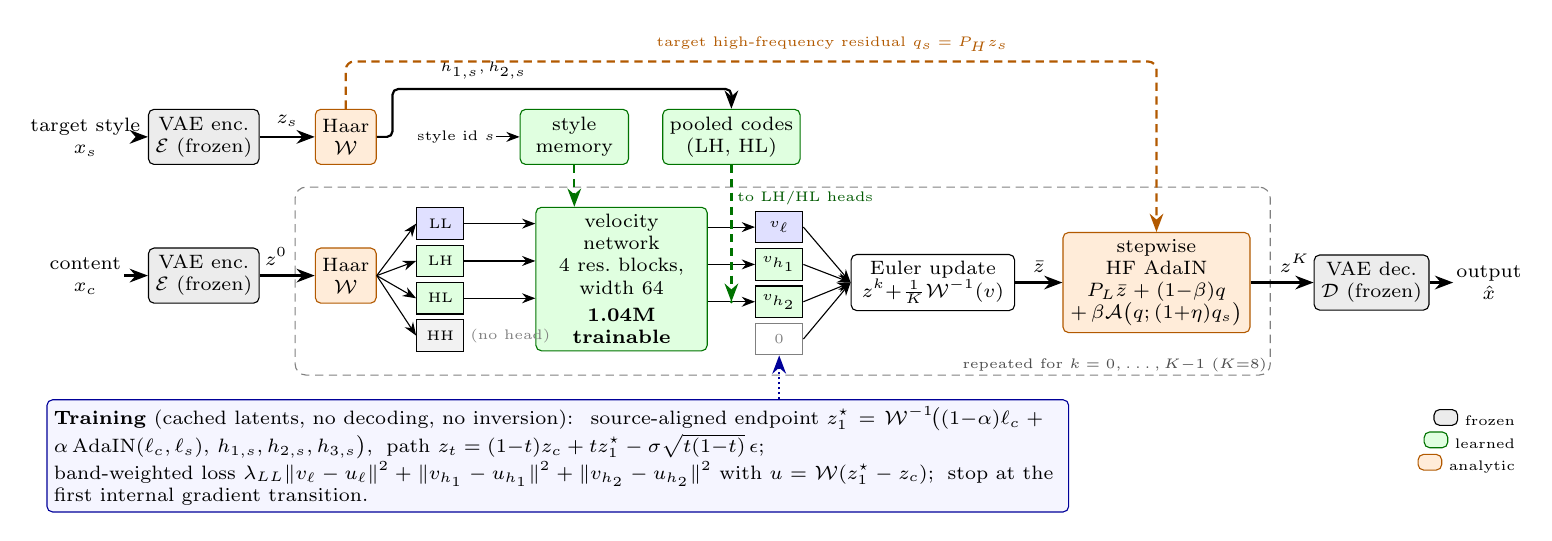
\begin{tikzpicture}[
  font=\scriptsize, >=Stealth, node distance=3mm,
  box/.style={draw, rounded corners=2pt, align=center, inner sep=2.5pt, minimum height=7mm},
  frozen/.style={box, fill=gray!15},
  learn/.style={box, fill=green!12, draw=green!45!black},
  analytic/.style={box, fill=orange!15, draw=orange!70!black},
  data/.style={align=center, inner sep=1pt},
  band/.style={draw, minimum width=6mm, minimum height=4mm, inner sep=0pt, font=\tiny},
  flow/.style={->, thick},
  cond/.style={->, densely dashed, orange!70!black, thick},
  lcond/.style={->, densely dashed, green!45!black, thick},
]
% ---------------- main inference path ----------------
\node[data] (xc) {content\\$x_c$};
\node[frozen, right=of xc] (enc) {VAE enc.\\$\mathcal E$ (frozen)};
\node[analytic, right=7mm of enc] (dwt) {Haar\\$\mathcal W$};
\node[band, fill=blue!12, right=5mm of dwt, yshift=6.6mm] (ll) {LL};
\node[band, fill=green!12, below=0.6mm of ll] (lh) {LH};
\node[band, fill=green!12, below=0.6mm of lh] (hl) {HL};
\node[band, fill=gray!10, below=0.6mm of hl] (hh) {HH};
\node[learn, right=9mm of lh, yshift=-2.3mm, minimum height=17mm, text width=20mm] (net)
  {velocity network\\4 res.\ blocks, width 64\\[2pt]\textbf{1.04M trainable}};
\node[band, fill=blue!12, right=6mm of net, yshift=6.6mm] (vll) {$v_\ell$};
\node[band, fill=green!12, below=0.6mm of vll] (vlh) {$v_{h_1}$};
\node[band, fill=green!12, below=0.6mm of vlh] (vhl) {$v_{h_2}$};
\node[band, draw=gray, text=gray, below=0.6mm of vhl] (vhh) {$0$};
\node[box, right=6mm of vlh, yshift=-2.3mm, text width=19mm] (euler)
  {Euler update\\$z^k{+}\tfrac1K\mathcal W^{-1}(v)$};
\node[analytic, right=6mm of euler, text width=22mm] (adain)
  {stepwise HF AdaIN\\$P_L\bar z+(1{-}\beta)q$\\$+\,\beta\mathcal A\big(q;(1{+}\eta)q_s\big)$};
\node[frozen, right=8mm of adain] (dec) {VAE dec.\\$\mathcal D$ (frozen)};
\node[data, right=of dec] (out) {output\\$\hat x$};

\draw[flow] (xc) -- (enc);
\draw[flow] (enc) -- node[above, pos=0.3]{$z^0$} (dwt);
\foreach \b in {ll,lh,hl,hh} \draw[->] (dwt.east) -- (\b.west);
\foreach \b in {ll,lh,hl} \draw[->] (\b.east) -- (\b.east -| net.west);
\node[font=\tiny, text=gray, anchor=west, inner sep=0.5pt] at ([xshift=0.5mm]hh.east) {(no head)};
\foreach \b in {vll,vlh,vhl} \draw[->] (\b.west -| net.east) -- (\b.west);
\foreach \b in {vll,vlh,vhl,vhh} \draw[->] (\b.east) -- (euler.west);
\draw[flow] (euler) -- node[above]{$\bar z$} (adain);
\draw[flow] (adain) -- node[above, pos=0.7]{$z^{K}$} (dec);
\draw[flow] (dec) -- (out);

\begin{scope}[on background layer]
\node[draw=black!50, densely dashed, rounded corners=4pt, inner sep=2.5mm,
      fit=(dwt)(ll)(hh)(net)(vll)(vhh)(euler)(adain)] (loop) {};
\end{scope}
\node[anchor=south east, font=\tiny, text=black!70, inner sep=1.2pt] at (loop.south east) {repeated for $k=0,\dots,K{-}1$ ($K{=}8$)};

\coordinate (mid) at ($(net.east)!0.5!(vlh.west)$);
% ---------------- style conditioning (top) ----------------
\node[data, above=12mm of xc] (xs) {target style\\$x_s$};
\node[frozen] (enc2) at (xs -| enc) {VAE enc.\\$\mathcal E$ (frozen)};
\node[analytic] (dwt2) at (xs -| dwt) {Haar\\$\mathcal W$};
\node[learn] (pool) at (xs -| mid) {pooled codes\\(LH, HL)};
\node[learn, text width=12mm] (mem) at ([xshift=-6mm]xs -| net) {style\\memory};
\draw[flow] (xs) -- (enc2);
\draw[flow] (enc2) -- node[above]{$z_s$} (dwt2);
\draw[flow, rounded corners=2pt] (dwt2.east) -- ++(2mm,0) |- ([yshift=2.5mm]mem.north) node[pos=0.75, above, font=\tiny]{$h_{1,s},h_{2,s}$} -| (pool.north);
\draw[lcond] (pool.south) -- (mid |- vhl.west);
\fill[green!45!black] (mid |- vlh.west) circle (0.6pt) (mid |- vhl.west) circle (0.6pt);
\node[font=\tiny, text=green!35!black, anchor=north west, inner sep=0.5pt] at ([xshift=0.5mm,yshift=-0.4mm]mid |- loop.north) {to LH/HL heads};
\draw[lcond] (mem.south) -- (mem.south |- net.north);
\node[font=\tiny, anchor=east, inner sep=0.5pt] (sid) at ([xshift=-3mm]mem.west) {style id $s$};
\draw[->] (sid) -- (mem);
\draw[cond, rounded corners=3pt] (dwt2.north) -- ++(0,6mm) -| node[pos=0.3, above, font=\tiny]{target high-frequency residual $q_s=P_H z_s$} (adain.north);

% ---------------- training objective (bottom) ----------------
\node[box, draw=blue!60!black, fill=blue!4, anchor=north west, text width=128mm, align=left]
  (loss) at ([yshift=-3mm]loop.south west -| xc.west)
  {\textbf{Training} (cached latents, no decoding, no inversion):\;
  source-aligned endpoint $z_1^\star=\mathcal W^{-1}\!\big((1{-}\alpha)\ell_c+\alpha\,\mathrm{AdaIN}(\ell_c,\ell_s),\,h_{1,s},h_{2,s},h_{3,s}\big)$,\;
  path $z_t=(1{-}t)z_c+t z_1^\star-\sigma\sqrt{t(1{-}t)}\,\epsilon$;\\
  band-weighted loss $\lambda_{LL}\|v_\ell-u_\ell\|^2+\|v_{h_1}-u_{h_1}\|^2+\|v_{h_2}-u_{h_2}\|^2$ with $u=\mathcal W(z_1^\star-z_c)$;\;
  stop at the first internal gradient transition.};
\draw[->, densely dotted, blue!60!black, thick] (loss.north -| vhh.south) -- (vhh.south);

\node[anchor=north east, font=\tiny, align=right] at (loss.north east -| out.east) {%
  \tikz\node[frozen, minimum height=2mm, minimum width=3mm]{};\ frozen\\[1pt]
  \tikz\node[learn, minimum height=2mm, minimum width=3mm]{};\ learned\\[1pt]
  \tikz\node[analytic, minimum height=2mm, minimum width=3mm]{};\ analytic};
\end{tikzpicture}
}
\caption{WEAVE. A one-level Haar transform exposes LL and three high-frequency bands of the VAE
latent. The compact network predicts LL/LH/HL velocities; pooled target LH/HL codes modulate only
the matching heads and HH has no learned head. After every Euler update, AdaIN aligns the combined
high-frequency residual to the target statistics. Only the green blocks are trained.}
\label{fig:framework}
\end{figure*}

\subsection{Latent Haar Coordinates}
Let $z_c=\mathcal E(x_c)\in\mathbb R^{4\times H\times W}$ and $z_s=\mathcal E(x_s)$ be content and
target-style latents of the frozen VAE. The one-level Haar transform
$\mathcal W(z)=(\ell,h_1,h_2,h_3)$ is orthonormal and exactly invertible, so losses and heads can be
assigned to explicit coordinates. We write $P_L z=\mathcal W^{-1}(\ell,0,0,0)$ and $P_H=I-P_L$;
latents with equal $P_L z$ share the LL coordinate but may differ in local appearance. Across
5{,}000 cross-style pairs, displacement energy concentrates in LL while style separability is
largest in HH (Fig.~\ref{fig:probes}): the band that dominates the regression is not the band that
carries style. The separation is exact in latent space, although the nonlinear decoder can still
couple visible structure and appearance.

\subsection{Source-aligned Endpoint}
A direct path from $z_c$ to $z_s$ also learns the unrelated geometry of $x_s$. WEAVE instead
keeps the source LL as an anchor and takes high frequencies from the target:
\begin{equation}
z_1^\star=\mathcal W^{-1}\big((1{-}\alpha)\ell_c+\alpha\,\mathrm{AdaIN}(\ell_c,\ell_s),\;h_{1,s},h_{2,s},h_{3,s}\big),
\label{eq:target}
\end{equation}
with $\alpha=0.3$, which permits a limited palette shift. Training samples a lightly perturbed
interpolation
\begin{equation}
z_t=(1{-}t)z_c+t z_1^\star-\sigma\sqrt{t(1{-}t)}\,\epsilon,\qquad u=z_1^\star-z_c,
\label{eq:path}
\end{equation}
with $t\sim\mathcal U[0,1]$, $\epsilon\sim\mathcal N(0,I)$, and $\sigma=0.02$. The perturbation
vanishes at both endpoints and is absent at inference; the label remains the clean displacement.

\subsection{Band-weighted Velocity Matching}
The network $v_\theta(z_t,t,s)$ predicts $(v_\ell,v_{h_1},v_{h_2})$ with separate $1{\times}1$ heads
on a shared trunk of four width-64 residual blocks. With $(u_\ell,u_{h_1},u_{h_2},u_{h_3})=\mathcal W(u)$,
\begin{equation}
\mathcal L=\mathbb E_t\big[\lambda_{LL}\|v_\ell-u_\ell\|^2+\|v_{h_1}-u_{h_1}\|^2+\|v_{h_2}-u_{h_2}\|^2\big],
\label{eq:loss}
\end{equation}
with $\lambda_{LL}=0.3$. Changing the endpoint (Eq.~\ref{eq:target}) alters the \emph{requested}
velocity, whereas $\lambda_{LL}$ alters its optimization pressure. A style memory indexed by the
target-style id gives a coarse prior to the trunk. For image-specific texture, the target LH and
HL bands are pooled into coordinate-free, orientation-specific codes that enter only the matching
heads; raw spatial target maps would leak target layout. HH has no learned head. The complete
model has 1{,}037{,}087 trainable parameters.

\subsection{Stepwise High-frequency Alignment}
Velocity matching organizes LL/LH/HL motion but leaves a weak appearance signal. For a residual
$q=P_H z$ and target residual $q_s=P_H z_s$, let
$\mathcal A(q;q_s)=\sigma(q_s)\,(q-\mu(q))/\sigma(q)+\mu(q_s)$ with channel-wise spatial
statistics~\cite{huang2017arbitrary}. One of $K$ inference steps is
\begin{equation}
\begin{aligned}
\bar z^{k+1}&=z^k+\tfrac1K\,\mathcal W^{-1}\big(v_\ell^k,v_{h_1}^k,v_{h_2}^k,0\big),\\
z^{k+1}&=P_L\bar z^{k+1}+(1-\beta)\,q^{k+1}+\beta\,\mathcal A\big(q^{k+1};(1+\eta)q_s\big),
\end{aligned}
\label{eq:step}
\end{equation}
with $q^{k+1}=P_H\bar z^{k+1}$, $K=8$, $\beta=2$, and $\eta=0.1$. Because $\beta>1$ the update
extrapolates toward the matched statistics; applying it at every step makes alignment part of
the dynamics rather than a post-process, and it supplies HH statistics without a learned head.

\subsection{Metric-free Stopping}
Training regresses a small latent field, needs no decoding, inversion, or adversary, and runs
52 steps per epoch at batch 96. After each epoch we probe a fixed batch of four latents at
$t=0.5$: $\rho_e$ is the ratio of LL to HF gradient norm on the shared trunk. Training stops at
the first epoch where the target-route gate grows and $\rho_e/\rho_{e-1}\le 0.65$, i.e., when
high-frequency learning takes over the trunk. On D5 this fires at epoch~4 (82.8\,s), which is
also the DINO-S peak of the 15-epoch curve; no external metric is used online.

\section{Experiments}
\label{sec:exp}

\subsection{Setup}
\noindent\textbf{Benchmarks.} \emph{D5-512}: five WikiArt styles (Early Renaissance,
Impressionism, Minimalism, Rococo, Ukiyo-e) at 512\,px, 3{,}600 training images each; 30 test
sources per style are sent to all five targets (750 ordered requests, same-style rows kept).
\emph{P2A-256}: a 256\,px grid over photo, Monet, Van Gogh, C\'ezanne, and Hayao.
\emph{R5-WikiArt}: five randomly drawn WikiArt families (Cubism, Expressionism, Pop Art,
Romanticism, Symbolism) at 512\,px.

\noindent\textbf{Metrics.} \dinos{} (primary) is the maximum cosine between the DINOv2-small
CLS feature~\cite{oquab2023dinov2} of the output and held-out references of the target style;
\clips{} is CLIP ViT-B/32~\cite{radford2021clip} similarity to the target-style prototype;
\dinoc{} is DINOv2 similarity to the source; LPIPS uses AlexNet. IDT and TGT (a fixed held-out
reference of the target style) are computed per board, and we inspect
$M_{\text{style}}(y)>M_{\text{style}}(y_{\text{IDT}})$ and
$\text{LPIPS}(y)<\text{LPIPS}(y_{\text{TGT}})$, $\dinoc(y)>\dinoc(y_{\text{TGT}})$ separately rather
than combining them into one score.

\noindent\textbf{Baselines and implementation.} We compare training-free diffusion editors
(SD-Turbo~\cite{sauer2023adversarial}, StyleAligned, Z-STAR, StyleShot, StyleID), learned models
(CUT, SaMST, SaMam, StyTR-2, AesPA-Net), the Seedream~4.5 API~\cite{seedream2025}, and an analytic
Latent-WCT, each at its released or recommended operating point. WEAVE uses AdamW (lr
$2\times10^{-4}$, cosine), bf16, and one RTX~3060 (12\,GB); training time excludes one-off latent
caching. Inference time covers the 8-step ODE and VAE decoding for 750 images.

\begin{table*}[t]
\centering
\caption{Main comparison (D-S: \dinos, C-S: \clips, LP: LPIPS, D-C: \dinoc). Excluding IDT and TGT,
the best entry per column is \textbf{bold} and the second \underline{underlined}. $\dagger$: style
not above IDT; $\ddagger$: content beyond TGT. Params in millions with frozen parameters as
superscript; Params and Train rank trained methods. WEAVE uses its selected D5 checkpoint on D5 and
dataset-specific checkpoints on P2A/R5; cost refers to the D5 model. Valid: number of benchmarks
without $\dagger$ or $\ddagger$. Times on one RTX~3060; $\ast$: author report on
four GPUs~\cite{deng2022stytr2}; $\sim$3\,h: Z-STAR estimated from step-scaled runs (full 512\,px runs exceed 12\,GB).}
\label{tab:main}
\scriptsize
\setlength{\tabcolsep}{2.1pt}
\renewcommand{\arraystretch}{0.95}
\resizebox{\textwidth}{!}{% Generated by tools/make_main_table.py from data/main_table.csv; do not edit by hand.
\begin{tabular}{@{}l*{12}{c}ccc@{}}
\toprule
& \multicolumn{4}{c}{D5-512} & \multicolumn{4}{c}{P2A-256} & \multicolumn{4}{c}{R5-WikiArt} & Params & Train & Infer \\
\cmidrule(lr){2-5}\cmidrule(lr){6-9}\cmidrule(lr){10-13}
Method & D-S$\uparrow$ & C-S$\uparrow$ & LP$\downarrow$ & D-C$\uparrow$ & D-S$\uparrow$ & C-S$\uparrow$ & LP$\downarrow$ & D-C$\uparrow$ & D-S$\uparrow$ & C-S$\uparrow$ & LP$\downarrow$ & D-C$\uparrow$ & (M) & (min) & (750) \\
\midrule
IDT (identity) & 0.419 & 0.693 & 0.000 & 1.000 & 0.416 & 0.663 & 0.000 & 1.000 & 0.433 & 0.731 & 0.000 & 1.000 & 0 & free & 0\,s \\
TGT (target style) & 1.000 & 0.863 & 0.776 & 0.215 & 1.000 & 0.835 & 0.800 & 0.169 & 1.000 & 0.796 & 0.747 & 0.230 & 0 & free & 0\,s \\
\midrule
SD-Turbo & 0.484 & 0.693$^{\dagger}$ & \textbf{0.003} & \textbf{0.922} & 0.341$^{\dagger}$ & 0.674 & 0.603 & 0.279 & 0.505 & 0.767 & 0.449 & 0.538 & 0$^{+1100}$ & free & 5\,m \\
StyleAligned & \textbf{0.675} & 0.780 & 0.869$^{\ddagger}$ & 0.239 & \textbf{0.612} & 0.768 & 0.786 & 0.310 & \textbf{0.649} & \textbf{0.824} & 0.829$^{\ddagger}$ & 0.315 & 0$^{+1100}$ & free & 77\,m \\
Z-STAR & 0.449 & 0.784 & 0.347 & 0.549 & 0.498 & \textbf{0.786} & 0.332 & 0.552 & 0.514 & \underline{0.822} & 0.384 & 0.526 & 0$^{+1100}$ & free & $\sim$3\,h \\
StyleShot & \underline{0.563} & \underline{0.787} & 0.765 & 0.377 & \underline{0.552} & \underline{0.774} & 0.713 & 0.335 & 0.484 & 0.787 & 0.795$^{\ddagger}$ & 0.380 & 0$^{+2400}$ & free & 5.1\,h \\
StyleID & 0.548 & \textbf{0.822} & 0.552 & 0.416 & 0.256$^{\dagger}$ & 0.648$^{\dagger}$ & 0.691 & 0.147$^{\ddagger}$ & \underline{0.551} & 0.815 & 0.493 & 0.385 & 0$^{+1100}$ & free & 63\,m \\
CUT & 0.471 & 0.714 & 0.374 & 0.795 & 0.539 & 0.754 & 0.494 & 0.702 & 0.441 & 0.710$^{\dagger}$ & 0.620 & \underline{0.795} & \underline{7.0} & 322.6 & 5\,m \\
SaMST & 0.271$^{\dagger}$ & 0.618$^{\dagger}$ & 0.749 & 0.145$^{\ddagger}$ & 0.501 & 0.709 & 0.398 & 0.838 & 0.461 & 0.667$^{\dagger}$ & 0.612 & 0.615 & 8.3 & \underline{39.5} & 10\,m \\
SaMam & 0.477 & 0.582$^{\dagger}$ & \underline{0.243} & \underline{0.812} & 0.505 & 0.677 & \textbf{0.205} & \textbf{0.870} & 0.503 & 0.712$^{\dagger}$ & \textbf{0.227} & \textbf{0.925} & 8.8 & 436.0 & 17.6\,m \\
StyTR-2 & 0.501 & 0.709 & 0.596 & 0.747 & 0.515 & 0.722 & 0.495 & 0.555 & 0.533 & 0.759 & 0.553 & 0.737 & 35.4$^{+12.9}$ & $\sim$1440$^{\ast}$ & 38\,m \\
AesPA-Net & 0.520 & 0.724 & 0.548 & 0.601 & 0.498 & 0.744 & 0.571 & 0.522 & 0.545 & 0.782 & 0.409 & 0.728 & 11.3$^{+20.0}$ & -- & 23\,m \\
Seedream 4.5 & 0.486 & 0.720 & 0.477 & 0.739 & 0.517 & 0.752 & \underline{0.227} & 0.785 & 0.504 & 0.742 & 0.486 & 0.725 & -- & API & -- \\
Latent-WCT & 0.362$^{\dagger}$ & 0.673$^{\dagger}$ & 0.441 & 0.559 & 0.338$^{\dagger}$ & 0.738 & 0.585 & 0.386 & 0.414$^{\dagger}$ & 0.710$^{\dagger}$ & 0.444 & 0.553 & 0 & free & \textbf{18\,s} \\
\midrule
\textbf{WEAVE (ours)} & 0.492 & 0.713 & 0.260 & 0.810 & 0.480 & 0.668 & 0.312 & \underline{0.861} & 0.523 & 0.775 & \underline{0.289} & 0.772 & \textbf{1.04$^{+84}$} & \textbf{1.4} & \underline{126\,s} \\
\bottomrule
\end{tabular}
}
\end{table*}

\subsection{Main Results}
\noindent\textbf{Auditing the field.} The last column of Table~\ref{tab:main} counts the benchmarks on
which a method stays inside the sandwich; only five of thirteen reach 3/3. The failures are
instructive. SD-Turbo attains the best D5 LPIPS (0.003) precisely because it barely edits the input:
its \clips{} equals that of IDT. SaMam, the strongest compact baseline on content, has \clips{} below
IDT on two benchmarks, so its low LPIPS partly reflects the identity shortcut. At the other extreme,
StyleAligned has the highest \dinos{} everywhere but moves farther from the source than an unrelated
target painting on D5 and R5. Latent-WCT never clears IDT, showing that wavelet statistics alone do
not produce transfer; the learned transport is necessary.

\noindent\textbf{Comparison among valid methods.} Restricted to the five methods that pass everywhere
(Z-STAR, StyTR-2, AesPA-Net, Seedream~4.5, and WEAVE), WEAVE has the highest \dinoc{} on all three
benchmarks (0.810/0.861/0.772) and the lowest LPIPS on D5 and R5, while its \dinos{} lies within the
range of the others. On D5 it reaches higher \dinos{} than the commercial Seedream~4.5 at about half
the LPIPS (0.260 vs.\ 0.477). The stronger D5-512 profile is consistent with native high-frequency
coefficients preserving detail that is compressed at 256\,px.

\noindent\textbf{Cost.} WEAVE has the fewest trainable parameters and the shortest training of all
learned methods (1.4\,min vs.\ 39.5--1440\,min, 28--1000$\times$ less) and needs 168\,ms per 512\,px
image including VAE decoding. Among the valid methods, the next cheapest learned model (AesPA-Net)
has 11$\times$ more trainable parameters and 11$\times$ longer inference.

\begin{figure*}[t]
\centering
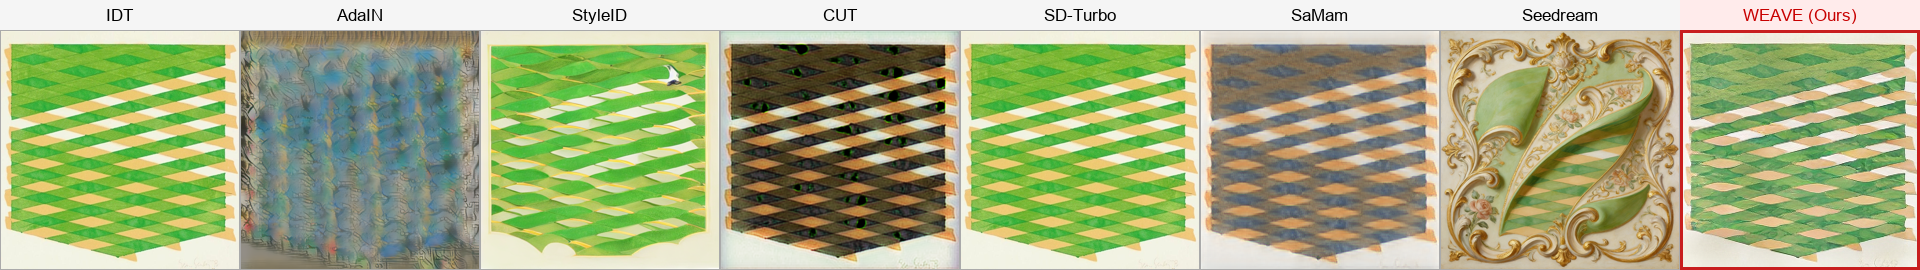
\includegraphics[width=\textwidth]{fig_teaser_comparison.png}
\caption{Extreme cross-domain request (Minimalism $\to$ Rococo). Diffusion editors substantially
alter source structure, and several lightweight or classical outputs remain close to identity.
WEAVE retains the source layout while adding the painterly target appearance.}
\label{fig:teaser}
\end{figure*}

\noindent\textbf{Qualitative comparison.} Fig.~\ref{fig:teaser} shows the same pattern visually:
editors that score high on style redraw the scene, compact baselines add color casts but little
texture, and WEAVE transfers brushwork onto the preserved source layout.

\subsection{Mechanistic Ablations}
Table~\ref{tab:ablation} changes one component at a time on the same 750 requests. Inference-time
controls reuse the selected checkpoint; retrained variants use seed 42 and are reported at their
best-\dinos{} epoch. Removing stepwise AdaIN lowers \dinos{} by 0.0097 and \clips{} by 0.0123 and moves the output
toward the source. Removing the high-frequency conditioning lowers \dinos{} and raises LPIPS.
Replacing the source-aligned endpoint with the direct target has the largest content cost (LPIPS
0.2595$\to$0.3138), and its peak arrives nine epochs later. Raising $\lambda_{LL}$ from 0.3 to 1.0
changes peak \dinos{} by less than 0.001 but lowers \dinoc{} to 0.787, so the method does not hinge
on a finely tuned weight. A learned HH head gives a small style gain for a small content cost, so
we keep the simpler model.

\begin{table}[t]
\centering
\caption{Component ablation on D5-512 (750 requests).}
\label{tab:ablation}
\footnotesize
\setlength{\tabcolsep}{4pt}
\begin{tabular}{@{}lcccc@{}}
\toprule
Variant & \dinos$\uparrow$ & \clips$\uparrow$ & LPIPS$\downarrow$ & \dinoc$\uparrow$ \\
\midrule
\textbf{WEAVE} (epoch 4) & 0.4918 & 0.7128 & 0.2595 & 0.8102 \\
w/o stepwise AdaIN ($\beta{=}0$) & 0.4821 & 0.7005 & 0.2258 & 0.8455 \\
w/o HF conditioning & 0.4825 & 0.7157 & 0.2837 & 0.8125 \\
direct endpoint ($z_1^\star{=}z_s$) & 0.4894 & 0.7172 & 0.3138 & 0.7966 \\
$\lambda_{LL}{=}1.0$ & 0.4910 & 0.7180 & 0.2626 & 0.7874 \\
learned HH head & 0.4930 & 0.7164 & 0.2670 & 0.8061 \\
\bottomrule
\end{tabular}
\end{table}

\subsection{Robustness and Transfer}
\noindent\textbf{Seeds and stopping.} The stopping rule selects epochs 4, 4, and 3 for seeds 42, 7,
and 123, giving \dinos{} 0.4918, 0.4910, and 0.4862 (LPIPS 0.260, 0.267, 0.255). For seeds 42 and 7,
where full 15-epoch curves exist, the selected epoch coincides with the \dinos{} peak.

\noindent\textbf{Reference pools.} Resampling a size-$m$ reference pool per target style 1{,}000 times,
the board-mean \dinos{} margin of WEAVE over IDT is positive in every draw: $0.030$ (95\% interval
$[0.020,0.039]$) for $m=8$ and $0.032$ ($[0.023,0.038]$) for $m=16$. About 69\% of individual
requests improve, so the claim is board-level rather than per image.

\noindent\textbf{Unseen families.} Applied without retraining to five held-out WikiArt families
(Table~\ref{tab:transfer}, top), the D5 checkpoint gives the best \clips{}, LPIPS, and \dinoc{};
SaMam is 0.015 higher on \dinos{} at a much higher LPIPS.

\noindent\textbf{Plug-in for a frozen editor.} We add the same Haar-domain alignment (LH/HL/HH,
scale 0.8, LL untouched) to a frozen SD1.5 image-to-image pipeline (empty prompt, strength 0.5,
20 DDIM steps). On 600 cross-style D5 pairs, \dinos{} and \clips{} rise significantly (paired
$t$-test, $p<10^{-15}$) at a small LPIPS change (Table~\ref{tab:transfer}, bottom), for 4.9\,ms per
image and no weight update.

\begin{table}[t]
\centering
\caption{Transfer beyond the training setting. Top: zero-shot on five unseen WikiArt families
(750 pairs, D5 checkpoints). Bottom: Haar alignment inside a frozen SD1.5 editor (600 pairs).}
\label{tab:transfer}
\footnotesize
\setlength{\tabcolsep}{4pt}
\begin{tabular}{@{}lcccc@{}}
\toprule
Method & \dinos$\uparrow$ & \clips$\uparrow$ & LPIPS$\downarrow$ & \dinoc$\uparrow$ \\
\midrule
SaMST & 0.3913 & 0.7485 & 0.6213 & 0.2680 \\
SaMam & \textbf{0.5466} & 0.7577 & 0.3990 & 0.7369 \\
WEAVE & 0.5313 & \textbf{0.7742} & \textbf{0.2802} & \textbf{0.7587} \\
\midrule
SD1.5 img2img & 0.3974 & 0.7221 & \textbf{0.3591} & \textbf{0.6589} \\
\;+ Haar alignment & \textbf{0.4080} & \textbf{0.7366} & 0.3630 & 0.6531 \\
\bottomrule
\end{tabular}
\end{table}

\section{Limitations and Conclusion}
\label{sec:conclusion}

WEAVE is evaluated with one SD1.5 VAE and a single Haar level; styles dominated by global palette
or layout, or expressed across several scales, may need a deeper decomposition. Haar separates
latent coordinates, not semantic factors, and the nonlinear decoder can couple them. The stopping
rule is validated on one architecture and three seeds, and IDT/TGT are board-specific references
measured with imperfect perceptual proxies. Baselines use their recommended operating points
rather than a compute-matched search.

The identity shortcut is easy to miss because the metrics that should catch it reward it. Two
trivial references, IDT and TGT, make it visible in raw metric units, and under them most of the
field fails somewhere. The shortcut has a spectral cause: coarse structure dominates the gradient
while carrying little style. WEAVE addresses that cause directly, anchoring structure at the
source, learning texture transport in explicit subbands, and injecting high-frequency statistics
along the trajectory. The result is the most content-preserving valid transfer we measured, from
a 1.04M-parameter model trained in 1.4 minutes on a consumer GPU, which makes style transfer
practical for resource-constrained multimedia applications. Code, checkpoints, and the
750-request protocol will be released; the supplement details the protocol, per-epoch curves,
and additional controls.

\bibliographystyle{IEEEbib}
\bibliography{refs}

\end{document}
